\chapter{Mushroom Rock Road}

\begin{enumerate}
	\item \sd, \cs. Walk back to guard to get \textbf{Tough Bangle}. Walk up, \sd, \sd.
	\item \textit{If you don't have \textbf{Self Destruct}, make sure that you get it before leaving the screen.}
	\item Flee from any encounters, go to the next screen.
	\item \save, go up the lift. Follow path.
	\item \formation{\tidus}{\wakka}{\auron}
\end{enumerate}
\begin{battle}{Non-Garuda Non-Ambush Anything}
	\begin{itemize}
		\switch{\tidus}{\kimahri}
		\kimahrif Defend
		\wakkaf Defend
		\switch{\auron}{\yuna}
		\summon{\valefor}
		\valeforf Energy Ray
	\end{itemize}
\end{battle}
\begin{enumerate}[resume]
	\item \formation{\tidus}{\wakka}{\auron}
\end{enumerate}
\end{multicols}
\newpage
\begin{multicols}{2}
\begin{spheregrid}
	\begin{itemize}
	\yunaf
	\begin{itemize}
		\item Use Magic Sphere
		\item +4 Magic
		\item Move to the right to +3 MagDef
		\item +3 MagDef, +3 Magic, +20 MP
		\item Move to Agil Node
		\item +3 Magic
	\end{itemize}
	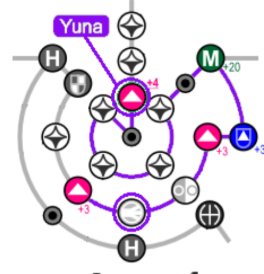
\includegraphics{graphics/yunammr}
	\kimahrif
	\begin{itemize}
		\item Move one right
		\item +200 HP
		\item Return to Lancet
		\item +200 HP
		\item Move to Agil node on the left
		\item +200 HP
	\end{itemize}
	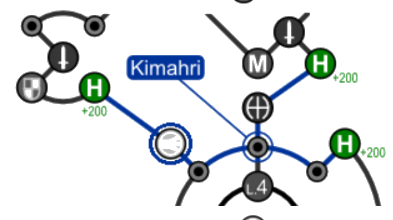
\includegraphics{graphics/kimahrimmr}
	\wakkaf
	\begin{itemize}
		\item Move to the HP node on the right
		\item +200 HP
		\item Move to Silence Attack on the right
		\item +2 Strength
	\end{itemize}
	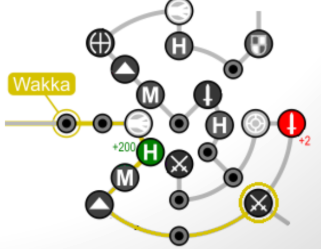
\includegraphics{graphics/wakkammr}
	\end{itemize}
\end{spheregrid}

\begin{encounters}
	\begin{itemize} % this can all be simplified down
		\item Raptor, Red Element, Gandarewa:
		\begin{itemize}
			\wakkaf Attack Raptor
			\switch{anyone}{\kimahri}
			\kimahrif Defend
			\switch{anyone}{\yuna}
			\summon{\valefor}
			\valeforf Boost
			\valeforf Blizzard Red Elemental
		\end{itemize}
		\item Raptor, Red Element, Fungar:
		\begin{itemize}
			\wakkaf Attack Raptor
			\switch{anyone}{\kimahri}
			\kimahrif Defend
			\switch{anyone}{\yuna}
			\summon{\valefor}
			\valeforf Fire Fungar
			\valeforf Boost
			\valeforf Blizzard Red Elemental
		\end{itemize}
		\item Raptor, Red Element, Lamashu:
		\begin{itemize}
			\wakkaf Attack Raptor
			\switch{anyone}{\kimahri}
			\kimahrif Attack Lamashtu
			\switch{anyone}{\yuna}
			\summon{\valefor}
			\valeforf Fire Lamashtu
			\valeforf Boost
			\valeforf Blizzard Red Elemental
		\end{itemize}
		\item Funguar, Red Element, Gandarewa:
		\begin{itemize}
			\wakkaf Attack Gandarewa
			\switch{anyone}{\kimahri}
			\kimahrif Defend
			\switch{anyone}{\yuna}
			\summon{\valefor}
			\valeforf Fire Funguar
			\valeforf Boost
			\valeforf Blizzard Red Elemental
		\end{itemize}
		\item Raptor, Red Element, Gandarewa:
		\begin{itemize}
			\wakkaf Attack Gandarewa
			\switch{anyone}{\kimahri}
			\kimahrif Attack Lamashtu
			\switch{anyone}{\yuna}
			\summon{\valefor}
			\valeforf Fire Lamashtu
			\valeforf Boost
			\valeforf Blizzard Red Elemental
		\end{itemize}
	\item Garuda: Flee
	\end{itemize}
\end{encounters}
\begin{enumerate}[resume]
	\item While Yuna still needs AP, do the following
\end{enumerate}
\begin{encounters}
	\begin{itemize}
		\wakkaf Attack Raptors or Gandarewas
		\switch{anyone}{\yuna}
		\yunaf Defend
		\item Flee
	\end{itemize}
\end{encounters}
\begin{enumerate}[resume]
	\item Make sure that you've completed the above sphere grid.
	\item \formation{\tidus}{\yuna}{\wakka}
	\item Go on lift, go to HQ. Go onto the main lift and onto the next screen.
	\item Walk down and \sd. Walk right to next screen, then right, \sd. Walk right to O'aka
\end{enumerate}
\begin{shop}{10890}
	\begin{itemize}
	\item Sell
	\begin{itemize}
		\item Hi-Potions
		\item Elixirs
		\item Tough Bangle
		\item Hunter's Spear
	\end{itemize}
	\item Buy
	\begin{itemize}
		\item Sentry, Equip
	\end{itemize}
	\end{itemize}
\end{shop}
\begin{enumerate}[resume]
	\item \sd, go right, \cs[1:00], \sd\ after Seymour. Go down to guard, confirm Yes, \sd
\end{enumerate}
\begin{battle}[12000]{Sinspawn Gui 1}
\begin{itemize}
	\tidusf Defend
	\switch{\yuna}{\auron}
	\auronf Power Break Main Body
	\wakkaf Switch Weapon to Thunder Ball or Official Ball
	\switch{\wakka}{\kimahri}
	\kimahrif Self Destruct main body
	\switch{\tidus}{\yuna}
	\summon{\valefor}
	\valeforf Energy Blast \od\ x2
	\item \textit{If \valefor\ doesn't charge second \od:}
	\begin{itemize}
		\valeforf Shield until Gui used a physical attack
		\valeforf Boost
		\valeforf Energy Blast \od
	\end{itemize}
\end{itemize}
\end{battle}
\begin{enumerate}[resume]
	\item \cs+\skippablefmv[2:20]. \sd\ Seymour dialogue.
\end{enumerate}
\begin{battle}[6000]{Sinspawn Gui 2}
\begin{itemize}
	\item \textbf{\textcolor{YellowGreen}{Seymour}}: Fira Head
	\item \textbf{\textcolor{YellowGreen}{Seymour}}: Fira Body x6
	\yunaf Defend
	\auronf Defend
\end{itemize}
\end{battle}
\begin{enumerate}[resume]
	\item \sd, \cs+\skippablefmv[2:00], walk left and up to Gatta, \sd. \fmv+\cs[1:30], \sd\ during \tidus\ monologue. \cs[1:00], \sd
	\item Walk left, \sd. Walk left, speak to \auron, \sd. Go up and right, \sd, exit area, \sd.
\end{enumerate}
\vfill
\ 
\columnbreak

